	\documentclass[
	%   draft,
	  a4paper,
	%   titlepage,
	  onecolumn,
	%  twocolumn,
	  11pt,
	  ]%
	% {scrartcl}%
	{article}%
	
	
	\usepackage[utf8x]{inputenc} 
	%\usepackage[utf8]{inputenc} % codificação deste ficheiro em UTF-8 
	
	\usepackage[T1]{fontenc}
	
	%% precisa ser carregado um outro tipo de letra por causa do efeito colateral do pacote T1:
	\usepackage{lmodern} % Fonte "Latin Modern" - A solução óptima para fontes latinas (resolve o problema do T1)
	% \usepackage{times}   % Fonte "Times"
	
	
	\usepackage{textcomp} % caracteres extra - símbolo do euro por exemplo
	
	% \usepackage[portuguese]{babel} % tradução portuguesa

	\newcommand{\referencesname}{Bibliografia}
	
	
	\renewcommand*\listfigurename{Indice de Figuras}
	
	%%%%%%%%%% Packages
	
	
	\usepackage[pdftex]{graphicx} % figuras 
	% \usepackage{subfigure} % subfiguras ( a,b,... )
	% \usepackage{wrapfig} % figuras ao lado de texto
	
	
	\usepackage{array} % mais opções nas tabelas (m{width}, b{width}, ...)
	\setlength{\extrarowheight}{1pt} % extra espaço entre as linhas das tabelas
	% \usepackage{multirow} % tabelas com células multilinha
	
	\usepackage{fancyhdr} % Estilo de página
	
		
	\usepackage[usenames,hyperref,pdftex%
	 ,svgnames%
	 ,x11names%
	 ,dvipsnames%
	%  ,cmyk
	 ]{xcolor} % Utilização de cores
	\usepackage{multicol}
	
	
	\usepackage[left=2.3cm,right=2.3cm,top=2.4cm]{geometry} % Margins
	
	
	% math packages by AMS
	\usepackage{amsmath} % main one
	
	
	

	\usepackage{fancyvrb} % more verbatim options 
	
		
	\usepackage[protrusion=true,expansion=true,stretch=10,shrink=10]{microtype} % micro-typographic extensions of pdfTEX (gets high quality text compostion)
	
	\usepackage[
	      pdftex,             %driver
	      colorlinks=true,    %no frame around URL
	      urlcolor=Black,    %no colors
	%       menucolor=black,    %no colors
	      linkcolor=black,    %no colors
	%       pagecolor=black,    %no colors
	      citecolor=Black,    %no colors
	      bookmarks=true,    %tree-like TOC
	      bookmarksopen=true,    %expanded when starting
	      bookmarksnumbered=true, %Put section numbers in bookmarks
	      hyperfootnotes=true,    %no referencing of footnotes, does not compile
	      pdfpagemode=UseOutlines,    %show the bookmarks when starting the pdf viewer
	      plainpages=false, %solve problem ``destination with the same identifier'' warning
	      pdfpagelabels %solve problem ``destination with the same identifier'' warning
	]{hyperref} % fazer hyperlinks (usar como último ``usepackage'')
	
	

	
	 \usepackage[colorinlistoftodos]{todonotes}
	
	\usepackage{xifthen}
	\usepackage{csvsimple}
	
	

	
	\newcommand{\tab}{\hspace*{2em}}
	
	%Text subscript
	\usepackage{fixltx2e}
	
	% Matrizes
	\usepackage{amsmath}
	
	%rename defaults
	
	\renewcommand{\figurename}{Figura}
	\renewcommand{\contentsname}{Indíce}
	\renewcommand{\abstractname}{Introdução}
	\renewcommand{\refname}{Referências}
	
	
	%Figure side by side
	
	\usepackage{subfig}
	
	%force float position
	\usepackage{float}
	\usepackage[section]{placeins}
	
	\makeatletter
	\AtBeginDocument{%
	  \expandafter\renewcommand\expandafter\subsection\expandafter{%
	    \expandafter\@fb@secFB\subsection
	  }%
	}
	\makeatother

	
	%Parametros de exibicao de codigo
	\usepackage{listings}
	\usepackage{color}
	
	\definecolor{mygreen}{rgb}{0,0.6,0}
	\definecolor{mygray}{rgb}{0.5,0.5,0.5}
	\definecolor{mymauve}{rgb}{0.58,0,0.82}
	
	
	
	
	%% Criação de comandos:
	\newcommand{\note}[1]{{\sffamily \slshape \textcolor{red}{#1}}}
	
	\colorlet{FPathColor}{Sepia}
	\colorlet{CmdColor}{blue}
	\colorlet{CmdRuleColor}{LightSteelBlue}
	\colorlet{FileTextColor}{DarkGreen}
	\colorlet{FuncColor}{DeepPink4}
	\CustomVerbatimCommand{\FPath}{Verb}{formatcom=\color{FPathColor},fontsize=\normalsize}
	\CustomVerbatimCommand{\Cmd}{Verb}{formatcom=\color{CmdColor},fontsize=\normalsize}
	\CustomVerbatimCommand{\FText}{Verb}{formatcom=\color{FileTextColor},fontsize=\normalsize}
	\CustomVerbatimCommand{\Func}{Verb}{formatcom=\color{FuncColor},fontsize=\normalsize}
	\DefineVerbatimEnvironment%
	  {Command}{Verbatim}
	  {formatcom=\color{CmdColor},frame=single,rulecolor=\color{CmdRuleColor},fontsize=\normalsize}
	\DefineVerbatimEnvironment%
	  {FileText}{Verbatim}
	  {formatcom=\color{FileTextColor},fontsize=\normalsize}
	
	
	% % Authors:
	
	
	
	\newcommand{\MYauthor}{Luís Rocha} 
	\newcommand{\MYnumber}{2010127532}
	
	\newcommand{\MYauthorII}{José Medeiros}
	\newcommand{\MYnumberII}{2010129934} 
	
		
	% % Titles:
	\newcommand{\MYtitle}{ROS - Detector de metais}
	\newcommand{\MYsubtitle}{Projecto} % Can be empty
	
	
	% % Course
	
	\newcommand{\MYcoursename}{Mecatrónica}
	\newcommand{\MYcourseyear}{2013/2014}
	
	
	% % PDF infos
	
	\newcommand{\MYkeywords}{} % Can be empty
	\newcommand{\MYsubject}{} % Can be empty
	
	
	%% Document format
	
	%% Fancy Headers
	\lhead{
\includegraphics[width=2cm]{logo_deec.pdf}}
	\chead{\sc\footnotesize Universidade de Coimbra\\
	Faculdade de Ciências e Tecnologia\\
	Departamento de Engenharia Electrotécnica e de Computadores}
	\rhead{
\includegraphics[width=0.8cm]{logo_fctuc.pdf}}
	\setlength{\headheight}{43pt}
	
	% Title
	\title{{\large\MYcoursename\ -- \MYcourseyear}\\[2mm]
	{\MYtitle}
	\ifthenelse{\equal{\MYsubtitle}{}}
	{\vspace*{1mm}}   {\\{\large\MYsubtitle}\vspace*{1mm}}
	}
	
	% Author / Number
	\author{%
	\MYauthor\\{\normalsize \href{mailto:ze_pedrom@hotmail.com}{\MYnumber}}
	\ifthenelse{\isnamedefined{MYauthorII}}
	{\and\MYauthorII\\{\normalsize \href{mailto:luis.rocha.jacinto@gmail.com}{\MYnumberII}}}    {}
	\ifthenelse{\isnamedefined{MYauthorIII}}
	{\and\MYauthorIII\\{\normalsize \href{mailto:a\MYnumberIII@alunos.deec.uc.pt}{\MYnumberIII}}}   {}
	}
	
	% Version / Date
	\date{%
	% \normalsize \today
	\mbox{}
	}
	


	
	
	%% PDF definitions:
	
	\hypersetup{%
	   pdftitle=\MYtitle,%
	   pdfauthor=\MYauthor,%
	%    pdfcreator=,%
	   pdfkeywords= {\MYkeywords},%
	%    pdfproducer=,%
	   pdfsubject= \MYsubject%
	} % informações do pdf (pacote hyperref)
	
	\pdfinfo{
	/Title	(\MYtitle)
	/Author (\MYauthor)
	/Keywords (\MYkeywords)
	} % informações do pdf
	
	\graphicspath{ {img/} } % Pasta das Imagens
	
	

	
	
	
	\begin{document}
	
	\maketitle
	\thispagestyle{fancyplain}
	
	\setlength{\parskip}{10pt}
	% Introdução
	 \begin{abstract} % (optional)
	
	 
	\tab Neste trabalho foi adaptado o robô Roomba para a detecção de minas terrestres.
	Foi utilizado o ROS (Robot Operating System) para fazer o controlo deste robô.
	Com o ROS foi possível controlar os movimentos do robô através do teclado usando um terminal.\\ \tab
	Para a detecção de minas foi utilizado o sensor \textit{LCD1000EVM}.
	\todo{Por os manuais do sensor}
	Este sensor devolve dois valores, o valor da proximidade e o valor da proximidade do metal. 
	Quando na presença de metais o valor da proximidade aumenta. Com base neste princípio é possível detectar a presença de minas.
	



	 
	 \end{abstract}
	
	
	\begin{figure}[ht]
	\centering
	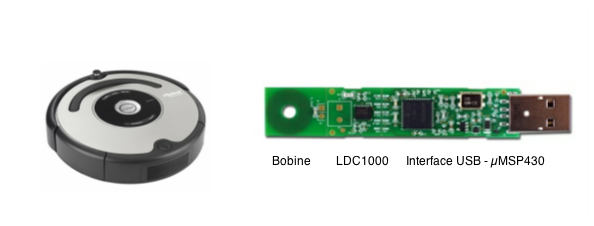
\includegraphics[width=140mm,scale=1]{im2.png}
	\caption{Roomba e Sensor LDC100EVM}\label{fig:cam}
	\end{figure}
	
	
	\newpage
	
	\listoftodos
	
	\newpage
	
        \tableofcontents
	
	\newpage
	
	\listoffigures

	
	\newpage
	
	
	
	\section{Descrição do problema}
	
	\tab Pretende-se detectar minas terrestres através do uso de um robô Roomba e de um sensor indutivo LCD1000EVM capaz de medir
	a proximidade e a frequência associada á presença de um metal nas imediações.
	Este sensor é composto por uma bobine em PCB, um LDC1000 que faz uso da bobine e um microcontrolador - MSP430. \\ \todo[color=brown!20]{Por a referencia da imagem que mostra isso}
	\tab Para ser possivel a concretização deste projecto é necessário implementar uma interface de comunicação entre
	o computador e o sensor para a aquisição de dados. Esta interface vai ser baseada num protocolo de comunicação que terá
	que ser o mesmo que é usado pelo microcontrolador. Será portanto necessário entender bem o protocolo visto que toda a base
	deste projecto se baseia neste sensor. \\
	\tab Após a interligação entre o sensor e o computador através de uma porta USB é necessário combinar o robô Roomba com o sensor utilizando a plataforma ROS \footnote{Distribuição Hydro}.
	Para isso é obrigatório fazer uso de transformadas ($tf's$) para referenciar o sensor ao eixo/referencial em relação ao referencial principal do robô. 
	Este passo é importantissimo para que se possa calcular as posições onde o sensor detecta minas.
	\todo[color=blue!20]{Dizer que mais abaixo vou explicar o conceito das tf's}

	
	\section{Conhecimentos Necessários}

	
	\tab Após analisarmos os requisitos deste projecto chegámos á conclusão de que era necessário familiarizarmos
	com a plataforma ROS. Sendo assim seguimos os tutoriais existentes no website WikiRos \cite{wikiros}.
	Após concluidos os tutoriais, ficamos aptos a usar ROS usando C++ como linguagem de programação. \\
	\tab Os seguintes conceitos/utilidades foram usados no nosso projecto, a sua explicação breve apresenta-se
	abaixo:
	
	
	
	
	
	
	\begin{description}
	    \item[Tf] \hfill \\
	  Estruturação dos referenciais do robô assim como as transformações necessárias entre os diferentes componentes \footnote{Sensores, plataformas, rodas, entre outros} do robô para que se possa saber as posições de qualquer elemento num dado instante. 
	    \item[Marker] \hfill \\
	  Estrutura de dados que permite usar as bibliotecas do \textit{rviz} para marcar minas no mapa. A posição das minas é obtida pela transformação da \textit{tf} do sensor em relação ao referencial base do robô.
	    \item[ArrayMarker] \hfill \\
	  Guardamos os markers (minas) que detectamos num array de markers. Para tal é necessário fazer \textit{push\_back} de um marker para o array quando é detectada a presença de uma mina.
	     \item[Serial Port] \hfill \\
	  Protocolo de comunicação usado para comunicar com o sensor através de uma porta USB.
	\end{description}
      

	
	
	
	
	
	\newpage
	
	\section{Material disponível}
	
	
	\begin{description}
	  \item[Robô e API] Roomba 555 com interface USB e \textit{Wrapper} para comunicar com o robô
	  \item[Sensor de Metal] LDC100EVM
	  \item[Computador] Portatil de pequenas dimensões com o sistema operativo Ubuntu\footnote{Ubuntu 13.04}
	  \item[Bobine] 1.5 mH
	  \item[Condensador] 19.2nF
	  \item[ROS] Plataforma ROS
	\end{description}


	
	
	\newpage
	\section{LDC100EVM}
	
	
	\tab O LDC100EVM é um sensor indutivo que permite medir a presença de metais retornando duas variavéis: posição do metal e a frequência de oscilação.
	É um circuito integrado que contém um microcontrolador MSP430 que é usado para fazer a interface entre
	o LDC (sensor) e um computador. 
	Este integrado vêm com uma bobine que pode ser mudada se se partir a PCB na zona a tracejado e colocando
	ai uma bobine á nossa escolha. É possivel ver na figura \ref{fig:sensor} a zona a tracejado:
	
	\begin{figure}[ht]
	\centering
	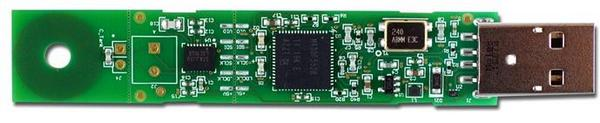
\includegraphics[width=140mm,scale=1]{im1.JPG}
	\caption{Zona a tracejado}\label{fig:sensor}
	\end{figure}
	
	
	Para dimensionar a bobine é necessário satisfazer duas condições para que o sensor possa funcionar na gama ideal:
	
	
	\begin{enumerate}
	  \item A freqência de ressonância deve estar compreendida entre 5 kHz e 5 MHz
	  \item A resistência de ressonância\footnote{Simboliza as perdas associadas ás correntes de Eddy} deve estar compreendida entre 798$\Omega$ e 3.93 M$\Omega$
	\end{enumerate}

	Para o calculo da freqência e a respectiva resistência usa-se as seguintes fórmulas:
	
	\begin{multicols}{2}
	
	\begin{equation}\label{freq_ress}
	 f_\text{ressonância} = \frac{1}{2\pi\sqrt{LC}}
	\end{equation}
	
	\begin{equation}\label{r_ress}
	 R_p = \frac{1}{R_s} \frac{L}{C}
	\end{equation}


	\end{multicols}
	
	
	Tendo em conta \eqref{freq_ress} e \eqref{r_ress} podemos dimensionar\cite{ldc1000evm} uma nova bobine para o sensor.
	Para garantir que a bobine juntamente com o novo condensador estão em contacto com o sensor
	deve-se soldar um adaptador na placa que permite a fácil colocação de elementos através de uma chave
	de fendas.
	
	
	
	
	Para calcular a indutância\cite{ldc1000_datasheet} medida pelo sensor é necessário fazer uso da frequência medida pelo LDC100EVM. Para tal:
	
	\begin{equation}
	 L_\text{medida} = \frac{1}{C* (2\pi f_\text{sensor})^2}
	\end{equation}

	
	
\href{run:./code/c++.cpp}{\color{RoyalBlue}Codigo C++} 

\href{run:./code/python.py}{\color{RoyalBlue}Codigo Python}

\href{run:./code/matlab.m}{\color{RoyalBlue}Codigo Matlab}

	
	\newpage
	\section{Solução proposta}
	
	
	
	\subsection{Hardware}
	
	\begin{figure}[ht]
	\centering
	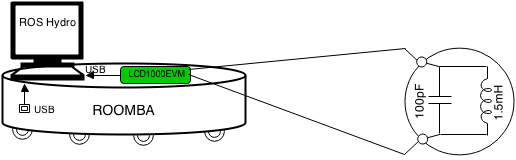
\includegraphics[width=150mm,scale=3]{roomba.png}
	\caption{Estrutura}\label{fig:roomba2}
	\end{figure}
	
	
	\subsubsection{Arquitectura}
	Em termos de hardware para este trabalho foi utilizado um computador que vai controlar o Roomba e o sensor LCD1000EVM.
	No sensor foi ainda substituída a bobine que vinha com o mesmo por uma bobine e um condensador de valores por nós pretendidos.
	
	\subsubsection{Implementação}
	O robô Roomba encontra-se conectado por usb a um computador que o controla.
	Este computador encontra-se ainda ligado a um sensor LCD1000EVM que por sua vez tem ligado a si uma bobine e um condensador por nós projectados e adaptados.
	
	\begin{figure}[ht]
	\centering
	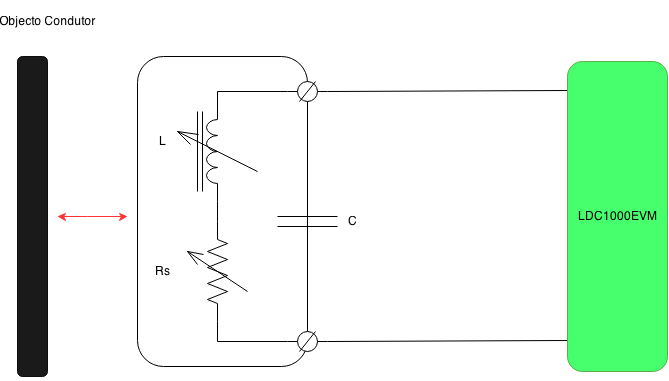
\includegraphics[width=150mm,scale=3]{circuito1.png}
	\caption{Circuito do Sensor}\label{fig:roomba3}
	\end{figure}
	
	Na presença de materiais conFdutores o valor de Rs e de L vão variar. Por intermédio da seguinte equação: \begin{equation}\label{rp}   
	R_p= \frac{1}{R_s}\times\frac{L}{C}
	\end{equation}  é possível aproximar o circuito da seguinte forma:
	
	
	\begin{figure}[ht]
	\centering
	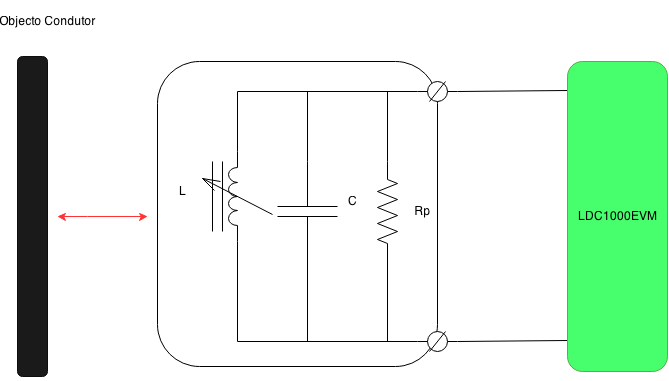
\includegraphics[width=150mm,scale=3]{circuito2.png}
	\caption{Circuito do Sensor}\label{fig:roomba4}
	\end{figure}
	\newpage
	Existe apenas uma condição para o bom funcionamento deste circuito com este sensor para: 
	
	
	\begin{equation}\label{Frequência}
	f_o = \frac{\omega_o}{2\pi} = \frac{1}{2 \pi \sqrt{LC}}
	\end{equation}
	
	 $f_o$ tem que estar compreendido entre 0.5Khz e 0.5Mhz. \\
Como tal desde que estas condições sejam cumpridas pode ser utilizada qualquer bobine, adaptando assim o sensor para diferentes situações por nós pretendidas. Tendo que ter em atenção que o sensor tem que se encontrar na gama de valores a cima referida, variando o valor do condensador garantimos que isso acontece.\\ \tab É apenas necessário a alteração dos registos da placa, para que estejam adequados ao novo circuito. Os registos a serem modificados são relativos ao $R_P$, mais especificamente ${R_P}_{MAX}$ e ${R_P}_{MIN}$ e à frequência $f_o$. O método mais simples para 

	\begin{figure}[ht]
	\centering
	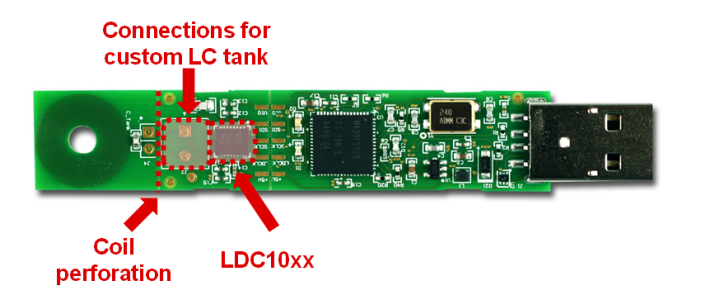
\includegraphics[width=150mm,scale=3]{circuito3.png}
	\caption{Circuito do Sensor}\label{fig:roomba5}
	\end{figure}
	\newpage
	
	
	\newpage
\section{Solução proposta: Software -Implementação}

\subsection{Utilização do ROS}

\tab Utilizámos o Robot Operating System (ROS) como plataforma de comunicação entre os dois periféricos por nós utilizados e o computador. Com o ROS é possível implementar bibliotecas de cliente ROS como roscpp, rospy ou roslisp. Por outras palavras significa que facilmente se consegue adaptar programas criados em outras línguas (de entre C++, Python e LISP). No nosso caso em específico adaptámos o programa de leitura do sensor em cpp para a plataforma ROS. Numa segunda parte através do api disponibilizado pelo Gonçalo Cabrita e pelo Bruno Gouveia conseguimos controlar o Roomba pelo teclado do computador. Através da leitura dos encoders e do controlo dos motores foi possível controlar a velocidade angular e linear do robô. \\ \tab Utilizando os nós do ROS foi possível assim controlar o robô e utilizá-lo para a deteção e marcação nas minas. De uma forma mais detalhada foi usada como referência a transformada "ODOM" que nos fornece a posição inicial em que o robô se encontra, com o nó entre esta transformada e o base link do Roomba sabe-se sempre a posição relativa à posição inicial. De seguida criando o nó da transformada sensor(criada por nós) é assim possível, com a informação devolvida pelo sensor, saber se o robô se encontra na presença de uma mina. Caso seja verificada a presença de uma mina são enviadas as coordenadas (x,y,z) para uma função "markers" que irá marcar no mapa as minas em relação a "ODOM", ou seja em relação à posição inicial do robô.

\subsection{Comunicação com o sensor}


\tab A primeira parte deste trabalho foi concluir que o sensor utiliza porta série como protocolo de comunicação quando comunica com o computador. Como tal, para facilitar o uso futuro deste sensor criámos código para as leituras do sensor em três plataformas diferentes de programação. Adaptámos por isso o nosso código às plataformas \textit{C++}, \textit{Matlab} e \textit{Python}. Estes três códigos encontram-se mais a baixo na tabela(Fazer referencia à tabela). \\ \tab Analisando as partes mais importantes do código, o primeiro passo é definir a porta série pela qual estamos a comunicar, no nosso caso em particular foi a porta "'COM9'". De seguida definimos o tipo de controlo de fluxo, que neste caso é do tipo "software flow control". É necessário definir a frequência de comunicação, Baud Rate, que foi definida por nós a 9600. O próximo passo é definir a paridade e o número de bits da comunicação, neste caso não existe paridade e são utilizados 8bits na comunicação. Tal como na maioria dos dispositivos electrónicos na comunicação por porta série apenas é necessário de 1 "stop bit", foi ainda definido o tempo de espera para leitura máximo("Timeout") a 5 segundos. Definimos o modo de leitura contínua para funcionar de forma assíncrona. Por fim ao escrever na porta série o comando 0x33(hexadecimal) ou 3(ASCII), iniciamos a stream de dados. 

	
	
	
	
	\section{Conclusões}
	

	\href{run:./code/a.cpp}{\color{RoyalBlue}Codigo C++}
         
       


	
	
	
	
	

	

\bibliographystyle{plain}
\bibliography{mylib}
	
	
\end{document}
